\documentclass[tikz,border=5mm]{standalone}
\begin{document}
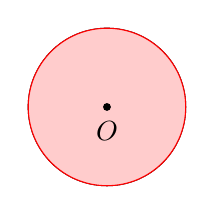
\begin{tikzpicture}
    % 绘制圆的轮廓
    \draw (0,0) circle (1cm);
    
    % 填充圆
    \filldraw[fill=red!20!white, draw=red] (0,0) circle (1cm);
    
    % 标注圆心
    \node [circle,fill=black,inner sep=1pt,label=below:$O$] at (0,0) {};
    
\end{tikzpicture}
\end{document}